\documentclass[a4paper,titlepage]{article}

\usepackage{graphicx}
\usepackage[italian]{babel}
\graphicspath{ {images/} }

\title{Relazione del Progetto Laboratorio di ASD\\[0.5em]
\large Prima Parte}
\date{Maggio 2021}
\author{
M. Giunta\thanks{Marco Giunta 147852 giunta.marco@spes.uniud.it} \and
S. Anzolin\thanks{Samuele Anzolin 111111 anzolin.samuele@spes.uniud.it} \and
F. Casani\thanks{Federico Casani 111111 casani.federico@spes.uniud.it} \and
G. De Nardi \thanks{Gianluca Giuseppe Maria De Nardi 142733 142733@spes.uniud.it}
}

\begin{document}
% Generate title page
\maketitle

% Generate TOC
\pagenumbering{arabic}
\tableofcontents
\newpage

\section{Introduzione}
In questo progetto abbiamo implementato e analizzato due algoritmi per il calcolo del periodo frazionario minimo di una stringa.
I due algoritmi implementati sono:

\begin{itemize}
  \item PeriodNaive
  \item PeriodSmart
\end{itemize}

Il linguaggio di programmazione che abbiamo utilizzato per questo progetto è C, in quanto è un linguaggio veloce ed efficiente e qualitativamente migliore per un’analisi temporale.

\section{Ipotesi}
Essendo periodNaive un algoritmo con complessità asintotica nel caso peggiore pari a O(\(n^2\)) mentre il secondo raggiunge una complessità lineare, possiamo dedurre
che periodSmart sarà notevolmente migliore nel caso peggiore.

\section{Implementazione}

\subsection{periodNaive}

L’implementazione di questo algoritmo come dice il suo nome, è abbastanza intuitiva.

Utilizziamo quindi un ciclo che scandisca l’intera stringa di input e internamente controlliamo la congruenza tra il prefisso e il suffisso precedentemente calcolato aumentando la lunghezza del bordo minimo man mano che il ciclo e il controllo avanzano.

\subsection{periodSmart}

Questo algoritmo invece, sfrutta il concetto di bordo, cioè una qualsiasi stringa che sia, prefisso e suffisso proprio della stringa principale.
Come osservato quindi p è un periodo frazionario di s solo se \(p = |s| - r\) dove r è la lunghezza di un bordo di s, quindi il problema si riduce al solo calcolo del bordo massimo della stringa s.

Andiamo quindi ad analizzare l’implementazione vera e propria del algoritmo in questione, avremo quindi:

\subsection{Algoritmo per il calcolo dei tempi medi}

Il calcolo dei tempi medi

\section{Analisi dei dati ottenuti}

\subsection{Grafico dei tempi di periodNaive}

\begin{figure}[h]
                \centering
                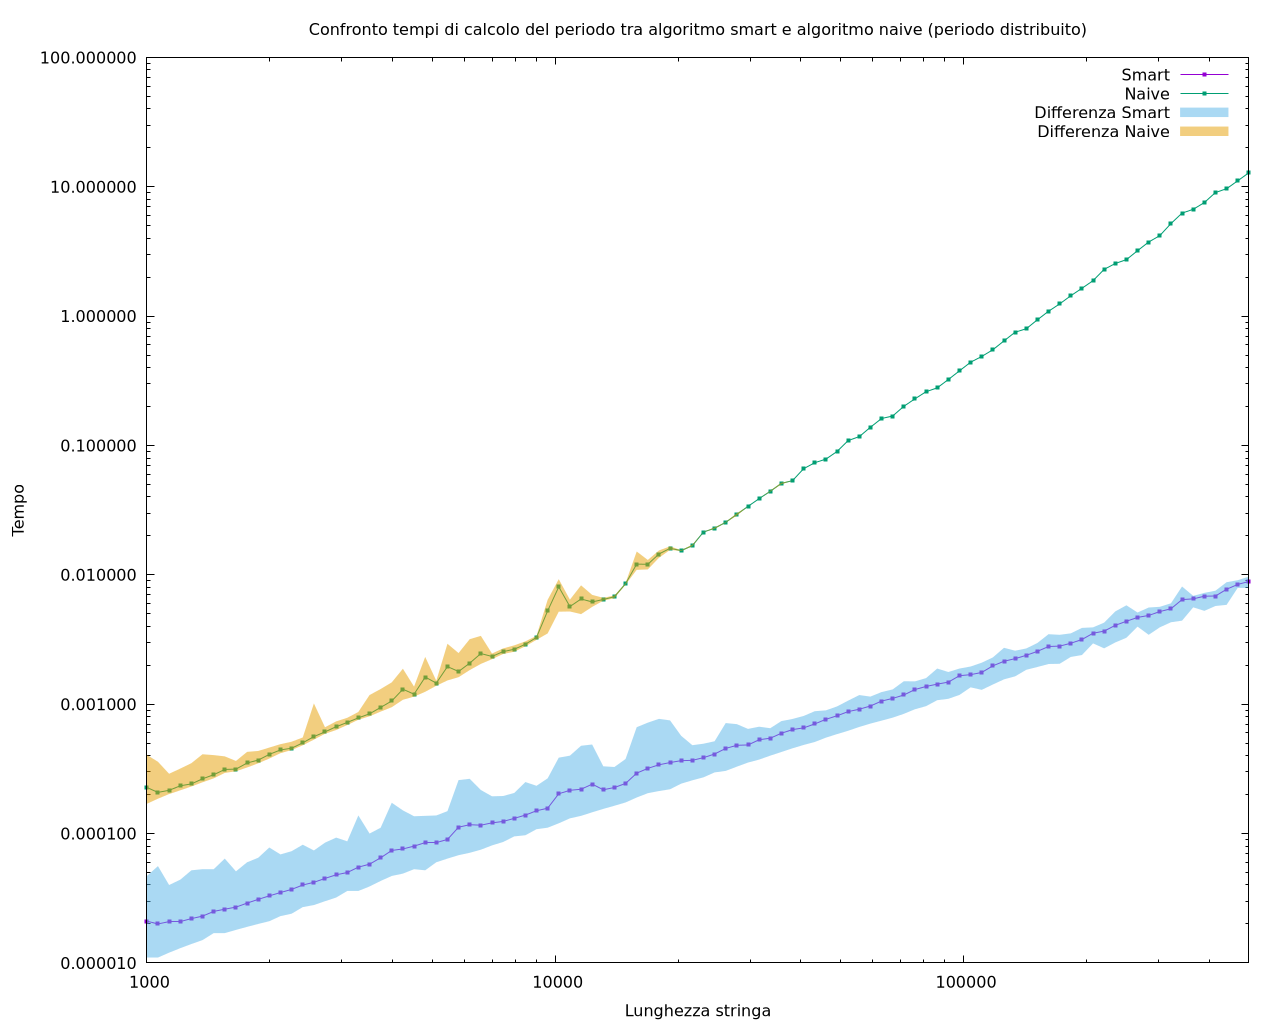
\includegraphics[width=\columnwidth]{test}
                \caption{Test}
                \label{fig:graph2}
\end{figure}



Allegare naive.pdf trasformato in immagine (ingrandire le scritte)

Allegare naivedist.pdf trasformato in immagine (ingrandire le scritte)

\subsection{Grafico dei tempi di periodSmart}

Allegare smart.pdf trasformato in immagine

Allegare smartdist.pdf trasformato in immagine

\subsection{Analisi logaritmica dei due algoritmi}

Allegare smartnaive.pdf trasformato in immagine

Non potendo analizzare i due algoritmi essendo su due scale temporali completamente differenti, dobbiamo quindi analizzarli in una scala logaritmica:

Allegare smartlog.pdf trasformato in immagine

Allegare naivelog.pdf trasformato in immagine

\subsection{Analisi comparativa tra i due algoritmi}

Allegare smart.pdf trasformato in immagine

Allegare naivedist.pdf trasformato in immagine

\section{Conclusioni}

Come osservato dai grafici, abbiamo sicuramente costatato che tra i due algoritmi c’è una notevole differenza in termini di tempo.
L’argoritmo smart impiega molto meno tempo dell'algoritmo rivale ed è quindi più consigliato il suo utilizzo.
\end{document}
